\documentclass[a4paper,10pt]{report}

\topmargin -2cm
%\topskip0cm
%\footskip0cm
%\headsep0cm
\parindent0cm
\oddsidemargin -1cm
\evensidemargin -1cm
\headheight 2cm
\textheight 24cm
\textwidth 18cm

\author{Alexander M\"unn (4403061)}
\title{\"Ubung}

\include{tex/header}
\usepackage{fancyhdr}
\pagestyle{fancy}
\lhead{Michael Borst\\ Alex Muenn}
\chead{"Ubungsblatt \nr\\\today}
\rhead{Computer Vision}



\newcommand{\nr}{1}

\begin{document}
\section*{Aufgabe 3 \& 4}

\begin{figure}[htpb]
\begin{center}
{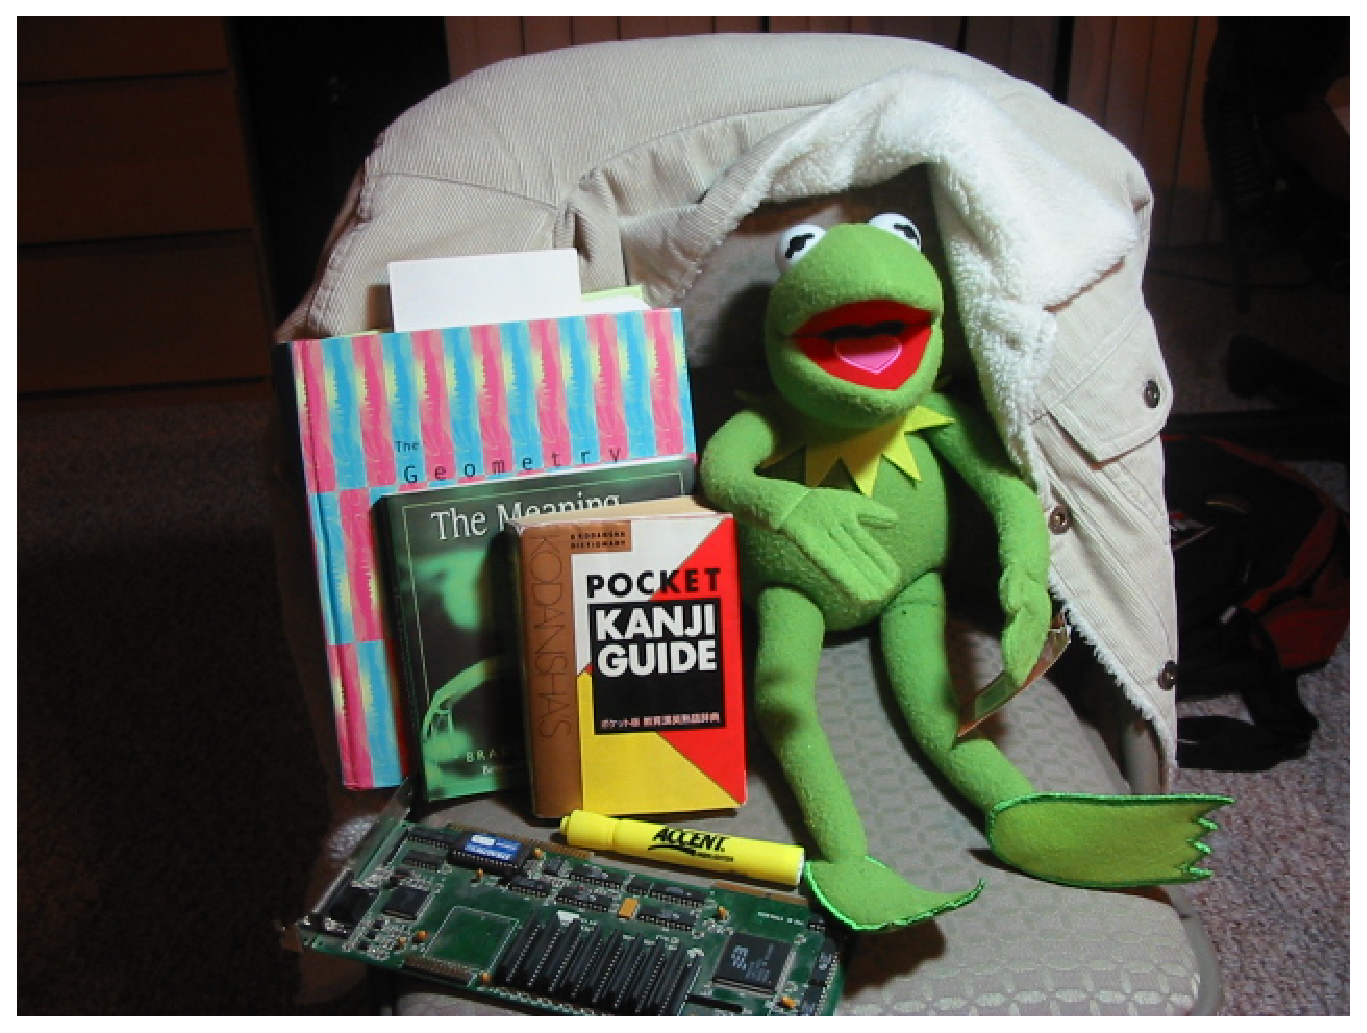
\includegraphics[width=0.25\textwidth]{samples/kermit001}}
\end{center}
\caption{Das Eingabebild für SIFT }
\label{fig:u02-picture}
\end{figure}

Folgende Funktion errechnet den (normierten) SIFT-Descriptor-Vektor.
Arbeitsschritte waren dabei Translation und Rotation des Koordinatensystems entsprechend dem Ort und der Orientierung des Descriptors, die Interpolation der Gradienten und dann die Aufteilung der Gradienten in die Bins der einzelnen Histogramme.

\lstset{language=matlab}
\begin{lstlisting}[caption={Berechnung des SIFT-Descriptor-Vektors}]
function SD = calculateSIFTDescriptor (Image, KeyPoint, rot, gridwidth, bsz, bins)
  # octave script to calculate sift descriptor for given keypoint

  [Dx, Dy] = gradient(Image, 0.5);

  step=2*pi/bins;


  SGx = zeros(gridwidth,gridwidth);
  SGy = SGx;
  # SIFT descriptor calculation needs its own coordinate system
  # compute x and y axis in image coordinate system
  #
  # +-----------> x
  # |
  # |  IMAGE
  # |  all angles are relative to top orientation (e.g. Vec(0 -1) has zero angle)
  # /
  # y
  #
  SDC_y = [-tan(rot*pi/180) 1];
  SDC_x = [1 tan(rot*pi/180)];
  SDC_x = SDC_x/norm(SDC_x);
  SDC_y = SDC_y/norm(SDC_y);
  # the origin of SIFT descriptor grid
  O = KeyPoint - (gridwidth/2-0.5)*(SDC_x+SDC_y);

  # fill grid with interpolated gradient information from origianl image gradients
  for y=1:gridwidth
    for x=1:gridwidth
      p = O + x*SDC_x + y*SDC_y;
      SGx(y,x) = gx = interp2(Dx,p(2), p(1));
      SGy(y,x) = gy = interp2(Dy,p(2), p(1));
      SG_magn(y,x) = norm([gx gy]);
    end
  end
  %-----------------------------------------------------------------------
  SG_theta = atan2(SGy, SGx) + pi;
  # unfortunatly SG_theta holds gradient angles in image space
  # we have to handle them relative to grids rotation
  SG_theta -= rot * pi/180;
  SG_theta = mod(SG_theta + 2*pi, 2*pi);
  # weight magnitude in the gaussian way
  g = gaussmatrix(gridwidth, gridwidth/2);
  SG_magn .*= g;

  SD = [];
  # 
  for b_y= 1:gridwidth/bsz
    for b_x = 1:gridwidth/bsz
      x=(b_x-1)*bsz+1;
      y=(b_y-1)*bsz+1;
      B_theta=SG_theta(x:x+bsz-1,y:y+bsz-1);
      B_magn=SG_magn(x:x+bsz-1,y:y+bsz-1);

      G_histo=zeros(1, bins);
      for row=1:bsz-1
        for col=1:bsz-1
          theta = B_theta(row,col);
          prevBin = floor(theta/step);
          nextBin = mod(prevBin+1,bins);
          prevBinDist = abs(prevBin*step-theta)/step;
          nextBinDist = 1-prevBinDist;
          mPrev = (1-prevBinDist)*B_magn(row,col);
          mNext = (1-nextBinDist)*B_magn(row,col);
          G_histo(uint8(prevBin+1)) += mPrev;
          G_histo(uint8(mNext+1))   += mNext;
        end
      end
      SD = [SD G_histo];
      # normalization of the feature vector
      SD = SD/norm(SD);
    end
  end
end
\end{lstlisting}



Folgende SIFT-Descriptoren wurden errechnet:

Aufgabe 3
\lstset{language=matlab}
\begin{lstlisting}[caption={Berechnung des SIFT-Descriptor-Vektors}]

\end{lstlisting}

Aufgabe 4
\lstset{language=matlab}
\begin{lstlisting}[caption={Berechnung des SIFT-Descriptor-Vektors}]
 Columns 1 through 6:

   1.1671e-04   4.2087e-05   0.0000e+00   0.0000e+00   0.0000e+00   0.0000e+00

 Columns 7 through 12:

   0.0000e+00   0.0000e+00   4.4894e-05   6.4458e-05   0.0000e+00   0.0000e+00

 Columns 13 through 18:

   0.0000e+00   0.0000e+00   0.0000e+00   0.0000e+00   3.3574e-04   0.0000e+00

 Columns 19 through 24:

   1.2298e-06   2.9508e-04   0.0000e+00   0.0000e+00   0.0000e+00   0.0000e+00

 Columns 25 through 30:

   2.1883e-04   0.0000e+00   0.0000e+00   2.8688e-05   0.0000e+00   2.8218e-05

 Columns 31 through 36:

   0.0000e+00   1.6973e-04   5.9733e-05   4.5022e-06   7.1678e-06   5.1812e-06

 Columns 37 through 42:

   2.3487e-06   1.8483e-06   4.6343e-06   6.6439e-06   7.9868e-05   1.3265e-05

 Columns 43 through 48:

   0.0000e+00   2.5081e-06   0.0000e+00   0.0000e+00   0.0000e+00   9.0657e-06

 Columns 49 through 54:

   6.5145e-04   0.0000e+00   0.0000e+00   5.0346e-04   0.0000e+00   0.0000e+00

 Columns 55 through 60:

   0.0000e+00   0.0000e+00   2.4477e-04   2.5645e-05   2.0481e-05   1.3771e-04

 Columns 61 through 66:

   0.0000e+00   0.0000e+00   0.0000e+00   5.6029e-05   2.7529e-05   0.0000e+00

 Columns 67 through 72:

   0.0000e+00   2.1178e-06   0.0000e+00   1.5833e-06   0.0000e+00   3.9622e-07

 Columns 73 through 78:

   4.8539e-05   8.6645e-06   0.0000e+00   8.0493e-06   1.2524e-08   4.7229e-07

 Columns 79 through 84:

   1.5133e-06   0.0000e+00   5.2351e-04   0.0000e+00   0.0000e+00   4.6291e-04

 Columns 85 through 90:

   0.0000e+00   0.0000e+00   0.0000e+00   0.0000e+00   4.9198e-04   0.0000e+00

 Columns 91 through 96:

   1.4505e-05   2.5375e-04   0.0000e+00   0.0000e+00   0.0000e+00   0.0000e+00

 Columns 97 through 102:

   2.9799e-05   8.7870e-06   0.0000e+00   1.0089e-06   9.8764e-06   0.0000e+00

 Columns 103 through 108:

   0.0000e+00   0.0000e+00   3.7551e-05   6.5017e-06   8.2781e-06   7.8495e-06

 Columns 109 through 114:

   3.8854e-07   1.5937e-06   0.0000e+00   0.0000e+00   4.4102e-04   0.0000e+00

 Columns 115 through 120:

   0.0000e+00   3.1684e-04   0.0000e+00   0.0000e+00   0.0000e+00   0.0000e+00

 Columns 121 through 126:

   3.7238e-04   0.0000e+00   0.0000e+00   2.9498e-04   0.0000e+00   0.0000e+00

 Columns 127 and 128:

   0.0000e+00   0.0000e+00
\end{lstlisting}

% \includegraphics[width=150mm]{<file.eps>}
\end{document}
